\documentclass[8pt, fleqn]{report}
\usepackage{amsmath, amssymb, ctex, geometry, graphicx, algorithm, algpseudocode}
\geometry{a4paper, total={7in, 9in}}
\author{R13621202}
\date{March 28}

\begin{document}
\section*{Exercise 1}

\subsection*{a}
\(n^{\frac{5}{6}}, \, 64^{\sqrt{n}}, \, n, \, \frac{\sqrt{n}}{\log^4 n}, \, n!, \, \log^{50} n, \, n^{\frac{6}{5}}, \, \log(n!), \, 4^n\)

\begin{itemize}
    \item 純對數的乘方 \(\log^{50} n\) 增長最慢。
    \item \(\dfrac{\sqrt{n}}{\log^4 n}\) 增長最終會超過單純的對數,但慢於任意正指數次方的 \(n^\alpha (\alpha > 0)\)。
    \item 對於 \(\log(n!)\),可寫為:
          \[
              \log(n!) = \sum_{k=1}^n \log k \leq \sum_{k=1}^n \log n = n \log n \quad \Rightarrow \quad \log(n!) = O(n \log n).
          \]
    \item 幾種多項式以指數大小排列:\(n^{\frac{5}{6}} < n < \log(n!) \approx n \log n < n^{\frac{6}{5}}\)。
    \item \(64^{\sqrt{n}} = 2^{6 \sqrt{n}}\),其增長比多項式快,但比 \(C^n\)(純指數函數)慢,因此有
          \[
              n^{\frac{6}{5}} < 64^{\sqrt{n}} < 4^n.
          \]
    \item 最後,\(n!\) 增長最快。
\end{itemize}

綜合以上,整體由小到大的排序為:
\[
    \log^{50} n < \frac{\sqrt{n}}{\log^4 n} < n^{\frac{5}{6}} < n < \log(n!) < n^{\frac{6}{5}} < 64^{\sqrt{n}} < 4^n < n!.
\]

\subsection*{b}

\subsubsection*{1. Prove or disprove: \(32^{\sqrt[3]{n}} = \Omega(4^n)\)}
假設 \(32^{\sqrt[3]{n}} \in \Omega(4^n)\),則存在常數 \(c > 0\) 與 \(n_0 > 0\),使得 \(\forall n \geq n_0, \quad 32^{\sqrt[3]{n}} \geq c \cdot 4^n\).

注意到 \(32 = 2^5\) 以及 \(4 = 2^2\),故不等式可改寫為 \(2^{5\sqrt[3]{n}} \geq c \cdot 2^{2n}\).

取對數後得到 \(5\sqrt[3]{n} \geq 2n + \log_2 c\).

由於當 \(n \to \infty\) 時,\(\sqrt[3]{n}\) 的增長遠慢於 \(n\),因此,對足夠大的 \(n\),不等式不成立,故 \(32^{\sqrt[3]{n}} \neq \Omega(4^n)\).

\subsubsection*{2. Prove or disprove: \(\sqrt{n}\log_2{n} = o(n)\)}
假設 \(\sqrt{n}\log_2{n} = o(n)\) 意味著對任一常數 \(c > 0\),存在 \(n_0 > 0\) 使得 \(\forall n \geq n_0, \quad \sqrt{n}\log_2{n} \leq c \cdot n\).

由於 \(\log_2{n} = 2\log_2\sqrt{n}\),不等式可改寫為 \(\frac{\log_2\sqrt{n}}{\sqrt{n}} \leq \frac{c}{2}\).

已知極限 \(\lim_{x \to \infty} \frac{\log x}{x} = 0\),令 \(x = \sqrt{n}\) 得 \(\lim_{n \to \infty} \frac{\log_2\sqrt{n}}{\sqrt{n}} = 0\).

因此,對足夠大的 \(n\),不等式成立,證明了 \(\sqrt{n}\log_2{n} = o(n)\).

\section*{Exercise 2}

\subsection*{a}
程式碼對於每個 \(i\)(從 1 到 \(n\)),內層迴圈執行 \(i^2\) 次,總執行次數為
\[
    \sum_{i=1}^{n} \sum_{j=1}^{i^2} 1 = \sum_{i=1}^{n} i^2 = \frac{n (n + 1) (2n + 1)}{6} = O(n^3).
\]

\subsection*{b}
程式碼對於每個 \(i\)(從 1 到 \(n\)),內層迴圈執行 \(2i + 1\) 次,將其加總
\[
    \sum_{i=1}^{n} (2i + 1) = 2 \sum_{i=1}^{n} i + \sum_{i=1}^{n} 1 = 2 \cdot \frac{n (n + 1)}{2} + n = n^2 + 2n = O(n^2).
\]

\section*{Exercise 3}

\subsection*{a}
使用 Recursive Tree method 來分析遞迴關係 \(T(n) = 2 \cdot T(n/4) + T(n/2) + n\),可以觀察到:

第 0 層:只有一個節點為根 (root),成本為 \(O(n)\).

第 1 層:共三個節點,分為兩個大小為 \(n/4\) 的子問題和一個大小為 \(n/2\) 的子問題,因此這一層的總成本為:
\[
    2 \cdot T(n/4) + T(n/2) + n = O(n).
\]

第 2 層:每個節點的大小進一步縮小,並且每層的額外工作(如 \(O(n)\))也會被計算。

這樣,我們可以看到在每一層,成本保持為 \(O(n)\).

\begin{center}
    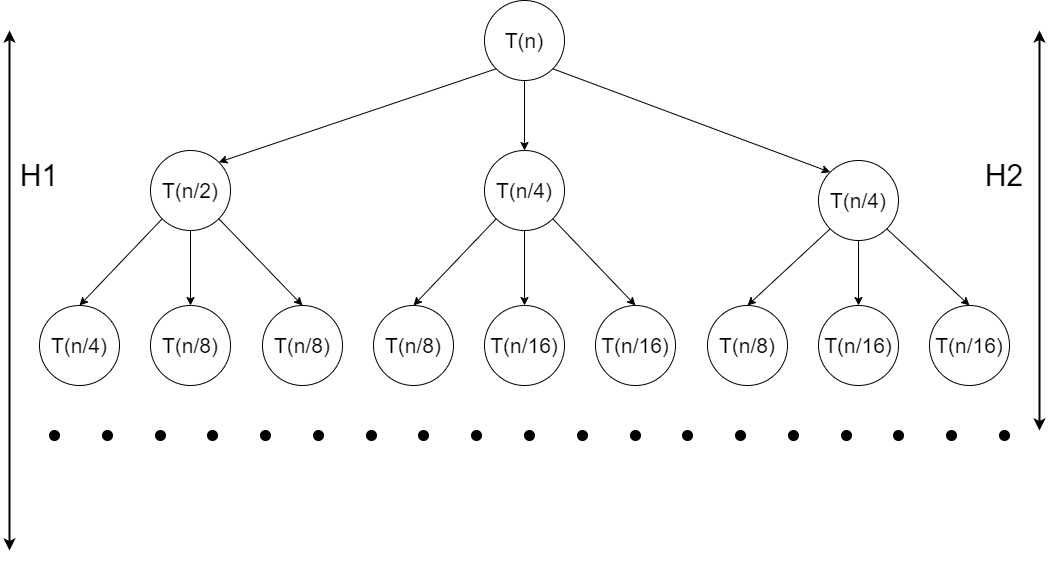
\includegraphics[width=60mm]{unbalance_case.png}
\end{center}

第一個節點完成的深度為 \(\log_4{n}\) (H2),所有節點都完成的深度為 \(\log_2{n}\) (H1).

因此時間複雜度的下界是 \(n \cdot \log_4{n} = \frac{1}{2} \cdot n \cdot \log_2{n}\),上界是 \(n \cdot \log_2{n}\).

上下界僅相差一個常數,可推論 \(T(n) = \Theta(n \cdot \log{n})\).

\subsection*{b}
使用 Master Theorem 分析 \(T(n) = 3 \cdot T(n/7) + \sqrt{n}\):

\(a = 3, \, b = 7, \, \log_b{a} = \log_7{3} \approx 0.564\),

\(f(n) = n^{1/2} \in O(n^{\log_7{3} - \varepsilon})\) where \(\varepsilon = 0.01\),

\(\Rightarrow\) Case 1,

\(\Rightarrow T(n) = \Theta(n^{\log_b{a}}) = \Theta(n^{\log_7{3}})\).

\subsection*{c}
先對 \(T(n) = 4 \cdot T(n^{\frac{1}{4}}) + \log_2{n}\) 做變數變換:

設 \(n = 2^m, \, n^{\frac{1}{4}} = 2^{\frac{m}{4}}\),

設 \(S(m) = T(2^m) = T(n) \Rightarrow S(\frac{m}{4}) = T(2^{\frac{m}{4}}) = T(n/4), \, f(n) = \log_2{2^m} = m\),

重寫 \(T(n) = S(m) = 4 \cdot S(\frac{m}{4}) + m\).

使用 Master Theorem 分析 \(S(m) = 4 \cdot S(\frac{m}{4}) + m\):

\(a = 4, \, b = 4, \, \log_b{a} = \log_4{4} = 1\),

\(f(m) = m \in \Theta(n^{\log_4{4}} \cdot \log{n}^k)\) where \(k = 0\),

\(\Rightarrow\) Case 2,

\(\Rightarrow S(m) = \Theta(m^{\log_b{a}} \cdot \log^{k+1}{m}) = \Theta(m \cdot \log{m})\),

轉變回 \(n\), \(T(n) = \Theta(\log{n} \cdot \log^2{n})\).

\section*{Exercise 4}
\(n\) 個數字下,每個數字被選為 pivot 的機率為 \(\frac{1}{n}\),對應的遞迴深度的期望值為:自己 1 層,加上 Pivot 左側的深度與 Pivot 右側的深度取最大值 (深度看最深的)。
\[
    \Pr[x = i] = \frac{1}{n}, \text{ and if } x = i, \, D(n) = \max (D(i-1) + D(n-i)) + 1.
\]

假設深度隨 \(n\) 增加而單調上升,且假設 \(x_1, x_2, \dots, x_{n-1}, x_n\) 為由小到大排好的序列,則:
\begin{align*}
     & x = 1: \quad D(n-1) + 1,                   \\
     & x = 2: \quad D(n-2) + 1,                   \\
     & \dots                                      \\
     & x = \frac{n}{2}: \quad D(\frac{n}{2}) + 1, \\
     & \dots                                      \\
     & x = n-1: \quad D(n-2) + 1,                 \\
     & x = n: \quad D(n-1) + 1.
\end{align*}

\[
    D(n) = 1 + \frac{2}{n} \sum_{i=\frac{n}{2}}^{n-1} D(i).
\]

在 Randomized QuickSort 中,Pivot 是均勻隨機挑選。平均而言,每次都會將陣列分成兩個大小大致相同的子陣列。對極大的 \(n\) 而言,\(D(i)\) 將以對數的形式成長,因此可以進一步將 \(D(n) \approx 1 + \frac{2}{n} \sum_{i=\frac{n}{2}}^{n-1} O(\log{i})\).

\begin{align*}
    D(n) & \approx 1 + \frac{2}{n} \sum_{i=\frac{n}{2}}^{n-1} \log{i} \\
         & = 1 + \frac{2}{n} \cdot n \log{n}                          \\
         & = 1 + 2 \log{n} = O(\log{n}).
\end{align*}

對於 Randomized QuickSort 在 \(n\) 個不同整數上的期望遞迴深度,隨著 \(n\) 的增長呈對數增長。因此,期望的遞迴深度為:\(D(n) = O(\log{n})\).

\section*{Exercise 5}
為了對 \(n\) 個數字進行排序,其中每個數字的位元長度為 \(o(\log_2{n})^2 = b\),可以使用 Radix Sort 來完成。從小位數到大進行排序,每一位數下的值範圍固定,可使用 counting sort 在線性時間內排完一個位數。

Radix Sort 的時間複雜度為:
\[
    T(n) = \Theta\left(\frac{b}{r}(n + 2^r)\right),
\]
其中 \(b\) 是每個數字的位元長度,\(r\) 是每次操作中所考慮的位數。我們希望在 \(o(n \log n)\) 時間內排序,根據問題的條件,\(b = o(\log_2{n})^2 > \lfloor \log_2{n} \rfloor\),因此我們可以選擇 \(r = \lfloor \log_2{n} \rfloor\),這樣能有效降低排序所需的時間。

選擇 \(r = \lfloor \log_2{n} \rfloor\) 使得時間複雜度變為:
\[
    T(n) = \Theta\left(\frac{b}{r}(n + 2^r)\right) = \Theta\left(\frac{b}{\log_2{n}}(n + n)\right) = \Theta\left(\frac{b \cdot n}{\log_2{n}}\right).
\]

由於 \(b = o(\log_2{n})^2\),可以得出:
\[
    T(n) = o\left(\frac{n \cdot (\log_2{n})^2}{\log_2{n}}\right) = o(n \log n).
\]

因此,這種排序方法可以在 \(o(n \log n)\) 時間內完成。

\section*{Exercise 6}
\(\langle x_1, x_2, \dots, x_n \rangle\): 排序好的 \(n\) 個 distinct number,

\(k\): 目標要找的數字排名,

定義 \(X_{i, j} (1 \leq i < j \leq n)\):
\begin{equation*}
    X_{i, j} = \begin{cases}
        1, & x_i \text{和 } x_j \text{ 在執行 QuickSelect 時比較過}, \\
        0, & \text{反之}.
    \end{cases}
\end{equation*}

\(E[x] = \sum_{i=1}^{n-1} \sum_{j=n+1}^{n} E[X_{i, j}]\).

假設 Pivot 是均勻隨機挑選。要使 \(i\) 和 \(j\) 被比較到,QuickSelect 在選擇 Pivot 時必須在特定範圍內先選到 \(i\) 或是 \(j\) 作為該範圍的第一個 Pivot。該範圍的值被選為 Pivot 的機率服從 \(Unif(a, b)\),選到 \(i\) 或 \(j\) 的機率為 \(\frac{2}{b-a+1}\)。以下分三個情境討論:

\textbf{Case 1: \(1 \leq k \leq i < j \Rightarrow a = k, \, b = j\)},

\textbf{Case 2: \(i < k < j \Rightarrow a = i, \, b = j\)},

\textbf{Case 3: \(i < j \leq k \leq n \Rightarrow a = i, \, b = k\)}.

\begin{flalign*}
    E[x] & = \sum_{j=k+1}^{n} \sum_{i=k}^{j-1} \frac{2}{j-k+1}                            \\
         & = \sum_{j=k+1}^{n} (j - k) \frac{2}{j-k+1}                                     \\
         & \leq 2 (n - k) \quad \forall j > k \, \left(\frac{j - k}{j - k + 1} < 1\right) \\
         & \leq 2n = O(n).
\end{flalign*}

\begin{flalign*}
    E[x] & = \sum_{j=k+1}^{n} \sum_{i=1}^{k-1} \frac{2}{j-i+1}                                                                                                                                                                    \\
         & = 2 \sum_{j=k+1}^{n} \frac{1}{j} + 2 \sum_{j=k+1}^{n} \frac{1}{j-1} + \dots + 2 \sum_{j=k+1}^{n} \frac{1}{j-k+2}                                                                                                       \\
         & = 2 \left(\frac{1}{k+1} + \frac{1}{k+2} + \dots + \frac{1}{n}\right) + 2 \left(\frac{1}{k} + \frac{1}{k+1} + \dots + \frac{1}{n-1}\right) + \dots + 2 \left(\frac{1}{3} + \frac{1}{4} + \dots + \frac{1}{n-k+2}\right) \\
         & = 2 (\ln{n} - \ln{k}) + 2 (\ln{n-1} - \ln{k-1}) + \dots + 2 (\ln{n-k+2} - \ln{2})                                                                                                                                      \\
         & = 2 \left(\ln{\frac{n}{k}} + \ln{\frac{n-1}{k-1}} + \dots + \ln{\frac{n-k+2}{2}}\right)                                                                                                                                \\
         & \leq 2 \left(\ln{\frac{n}{k}} + \ln{\frac{n-1}{k-1}} + \dots + \ln{\frac{n-k+2}{2}} + \ln{\frac{n-k+1}{1}}\right)                                                                                                      \\
         & = \ln{\frac{n(n-1)(n-2)\dots(n-k+1)}{k(k-1)(k-2)\dots3\cdot2\cdot1}}                                                                                                                                                   \\
         & = \ln{\binom{n}{k}}                                                                                                                                                                                                    \\
         & \leq \ln{2^n} = n \ln{2} = O(n).
\end{flalign*}

\begin{flalign*}
    E[x] & = \sum_{j=i+1}^{k} \sum_{i=1}^{j-1} \frac{2}{k-i+1}                            \\
         & = \sum_{i=1}^{j-1} (k - i) \frac{2}{k-i+1}                                     \\
         & \leq 2 (j - 1) \quad \forall k > i \, \left(\frac{k - i}{k - i + 1} < 1\right) \\
         & \leq 2j \leq 2n = O(n).
\end{flalign*}

在所有情境下,QuickSelect 的期望時間複雜度皆為 \(O(n)\).

\section*{Exercise 7}
\begin{algorithm}[H]
    \caption{FindMinEnergy (\textit{n, Obstacles})}
    \label{alg:FindMinEnergy}
    \begin{algorithmic}[1]
        \For{$i = 1$ \textbf{to} $n$}
        \State $me[i] \gets \infty$ \Comment{Initialize the me array}
        \EndFor
        \State $me[0] \gets 0$ \Comment{No energy is required to start at position 0}
        \For{$i = 0$ \textbf{to} $n$}
        \If{$me[i] \neq \infty$} \Comment{Only consider reachable positions}
        \If{$(i + 1) \leq n$ \textbf{and} $(i + 1) \notin Obstacles$} \Comment{Try to walk to i + 1}
        \State $me[i + 1] \gets \min(me[i + 1], me[i] + 1)$ \Comment{Updates the minimum energy required to reach position i + 1}
        \EndIf
        \If{$(i + 4) \leq n$ \textbf{and} $(i + 4) \notin Obstacles$} \Comment{Try to jump to i + 4}
        \State $me[i + 4] \gets \min(me[i + 4], me[i] + 6)$ \Comment{Updates the minimum energy required to reach position i + 4}
        \EndIf
        \EndIf
        \EndFor
        \State \Return $me[n]$
    \end{algorithmic}
\end{algorithm}

初始化位置所需能量陣列:從 1 迭代至 \(n\),每次迭代使用常數時間 \(O(1)\) 將位置 \(i\) 的值指定為無限大,時間複雜度 \(O(n)\)。指定位置 0 的所需能量為 0,時間複雜度為 \(O(1)\)。因此初始化的時間複雜度為 \(O(n) + O(1) = O(n)\).

更新位置所需能量:從 0 迭代至 \(n\),對於每個位置 \(i\),都會檢查該位置是否可抵達。如果可以,則會考慮兩種可能的移動:
1. 走到 \(i + 1\)(如果它不是障礙物並且不大於 \(n\));
2. 跳到 \(i + 4\)(如果它不是障礙物並且不大於 \(n\))。嘗試不同的移動方式都可能更新位置所需的最小能量。檢查和更新都是在常數時間 \(O(1)\) 下完成。迭代 \(n + 1\) 次,每次迭代執行時間 \(O(1)\),因此時間複雜度為 \(O(n)\).

回傳 \(n\) 位置的能量值:在常數時間 \(O(1)\) 完成操作。

演算法的總體時間複雜度為 \(O(n) + O(n) + O(1) = O(n)\).

\section*{Exercise 8}
\begin{algorithm}[H]
    \caption{FindLPS (\textit{seq})}
    \label{alg:FindLPS}
    \begin{algorithmic}[1]
        \State $n \gets \textbf{length(seq)}$ \Comment{Get the length of the input sequence}
        \For{$i = 2$ \textbf{to} $n$}
        \For{$j = i-1$ \textbf{to} $1$}
        \State $ps[i][j] \gets 0$ \Comment{Initialize the ps array}
        \EndFor
        \EndFor
        \For{$i = 1$ \textbf{to} $n$}
        \State $ps[i][i] \gets 1$ \Comment{Set the diagonal of ps to 1 (single character palindromes)}
        \EndFor
        \For{$i = 2$ \textbf{to} $n$}
        \For{$j = i-1$ \textbf{to} $1$}
        \If{$seq[i] = seq[j]$}
        \State $ps[i][j] \gets 2 + ps[i-1][j+1]$ \Comment{If characters match, extend palindrome length}
        \Else
        \State $ps[i][j] \gets \max{ps[i-1][j], ps[i][j+1]}$ \Comment{Otherwise, take the max length from neighbors}
        \EndIf
        \EndFor
        \EndFor
        \State \Return $ps[n][0]$ \Comment{Return the length of the longest palindromic subsequence}
    \end{algorithmic}
\end{algorithm}

取得序列長度:這個步驟只需進行一次,且為常數時間操作 \(O(1)\).

初始化 \(ps\) 陣列:第一個迴圈,\(i\) 從 2 迭代到 \(n\),對於每個 \(i\),內部的迴圈從 \(j = i-1\) 迭代到 1,總共需要執行 \(\sum_{i=2}^{n} (i-1) = \sum_{i=1}^{n-1} i = \frac{(n-1)(n-2)}{2}\) 次操作,因此,這部分的時間複雜度是 \(O(n^2)\)。第二個迴圈,將對角線 \(ps[i][i]\) 設定為 1,這個步驟是從 \(i = 1\) 迭代到 \(n\),每次操作的時間是常數 \(O(1)\),總計為 \(O(n)\)。因此,初始化 \(ps\) 陣列的總時間複雜度是:\(O(n^2) + O(n) = O(n^2)\).

計算最長回文子序列長度:外層迴圈 \(i\) 從 2 到 \(n\),內層迴圈 \(j\) 從 \(i-1\) 到 1。對於每個 \(i\),內部的迴圈從 \(j = i-1\) 迭代到 1,總共需要執行 \(\sum_{i=2}^{n} (i-1) = \sum_{i=1}^{n-1} i = \frac{(n-1)(n-2)}{2}\) 次。對於每一組 \((i, j)\),程式根據 \(seq[i]\) 和 \(seq[j]\) 的相等情況來決定 \(ps[i][j]\) 的值。每次的操作為常數時間 \(O(1)\),因此這部分的總時間複雜度為 \(O(n^2)\).

返回結果:返回 \(ps[n][0]\) 的操作是常數時間操作 \(O(1)\).

因此,整個算法的總時間複雜度是由初始化 \(ps\) 陣列和計算最長回文子序列的部分主導,最終為:\(O(1) + O(n^2) + O(n^2) + O(1) = O(n^2)\).

\end{document}